\chapter{Kiến thức nền tảng}
\label{Chapter2}

Trong chương này, đầu tiên nhóm chúng em trình bày về thuật toán ``Matrix factorization'' - thuật toán đề xuất sản phẩm bằng cách phân rã ma trận tương tác. Sau đó nhóm chúng em sẽ trình bày về thuật toán ``Gradient descent'' - thuật toán mà nhóm chúng em sẽ sử dụng để cực tiểu hóa hàm chi phí của  ``Matrix factorization''. Ngoài ra, nhóm chúng em còn trình bày về ``Naive bayes'' và ``Logistic regression'' - hai mô hình phân lớp mà nhóm chúng em sẽ sử dụng để tìm ma trận xu hướng trong IPS. Chương này, đặc biệt là về phần ``Matrix factorization'' cung cấp những kiến thức nền tảng để có thể hiểu rõ về những cải tiến mà nhóm em tìm hiểu ở chương kế tiếp.

\section{``Matrix factorization''}
``Matrix factorization'' là một phương pháp thuộc nhóm lọc cộng tác (collaborative filtering), một nhóm các phương pháp tập trung vào mối quan hệ giữa các người dùng dựa trên đánh giá của các người dùng trong hệ thống. 
Phương pháp ``Matrix factorization'' sẽ phân tích ma trận tương tác $R \in \mathbb{R}^{m \times n}$ thành tích của hai ma trận $P \in \mathbb{R}^{m \times k}$ và $\mathbf{W} \in \mathbb{R}^{k \times n}$ (hình \ref{fig:chap2_MF1} mình họa về việc phân tách ma trận tương tác $R$), trong đó: $P$ và  $Q$ là ma trận đặc trưng của người dùng và sản phẩm; $k$ là hyperparameter được điều chỉnh trong quá trình huấn luyện mô hình, đại diện cho kích thước của đặc trưng tiềm ẩn.

\begin{figure}[h]
    \centering
    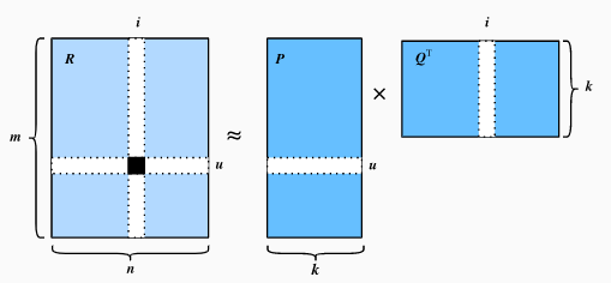
\includegraphics[width = \textwidth]{Chapter2/MF1.png}
    \caption{Matrix Factorization. Ma trận tương tác $R$ sẽ được phân rã thành ma trận đại diện cho người dùng $P$ và đại diện cho sản phẩm $Q$}
    \label{fig:chap2_MF1}
\end{figure}

Ma trận tương tác $R$ là ma trận thưa có kích thước là $m \times n$ chứa đánh giá của $m$ người dùng đối với $n$ sản phẩm có trong hệ thống. Đánh giá của người dùng $u$ cho sản phẩm $i$ trong ma trận tương tác sẽ được kí hiệu là $R_{u,i}$. Trong ma trận $P$ hàng thứ u sẽ được kí hiệu là $p_u$ và hàng thứ i trong ma trận $Q$ sẽ được kí hiệu là $q_i$.

Các đặc trưng tiềm ẩn trong $k$ mô tả sự liên quan giữa các người dùng và sản phẩm. Ví dụ như trong hệ thống đề xuất phim, các đặc trưng tiềm ẩn có thể là thể loại, ngôn ngữ, diễn viên hay bất kì các đặc trưng nào khác; hoặc có thể là bất cứ sự liên quan giữa người dùng và sản phẩm nào đó mà ta không thể giải thích được.
Mỗi sản phẩm $i$ trong ma trận sản phẩm $Q$ sẽ mang đặc trưng ẩn ở một mức độ nào đó tương ứng với các hệ số trong véc-tơ $q_i$ của nó, hệ số càng cao tương ứng với sản phẩm $i$ mang đặc trưng đó càng lớn. Tương tự, mỗi người dùng $u$ trong ma trận người dùng $P$ sẽ thích các đặc trưng ẩn này theo một mức độ nào đó tương ứng với các hệ số trong véc-tơ $p_u$, hệ số càng cao tương ứng với người dùng $u$ sẽ càng thích các bộ phim mang đặc trưng đó. Vì vậy, mục tiêu của chúng ta là sẽ đề xuất
cho người dùng $u$ những sản phẩm $i$ mang đặc trưng mà người dùng $u$ thích, tương ứng với giá trị của $p_u$ và $q_i$ đều cao dẫn đến $p_u \times q_i$ càng cao.









\section{``Gradient descent''}


\section{``Naive bayes''}


\section{``Logistic regression''}

